% For the listing caption reference
%! Suppress = UnresolvedReference

% To include word count of tables
%TC:group table 0 1

\chapter{Implementing Flexible Resource Allocation Environment and Server Agents}
\label{ch:implementing-flexible-resource-allocation-environment-and-server-agents}
To test the effectiveness of the proposed optimisation problem and agents from
Chapter~\ref{ch:optimising-resource-allocation-in-mec} a Mobile Edge Cloud
(MEC) computing network must be simulated for both training and evaluation of agents. However as this is impractical to
physically setup such a network to train agents in parallel and offline such a system must be simulated. \\
This chapter implements a simulation of MEC
networks (Section~\ref{sec:simulating-mec-networks}), server auction and resource
allocation agents (Section~\ref{sec:server-auction-and-resource-allocation-agents}) and the training of agents
(Section~\ref{sec:training-agents}).

The implementation discussed below is written in Python and available to download from
Github~\footnote{\url{https://github.com/stringtheorys/Online-Flexible-Resource-Allocation}}.

\section{Simulating MEC Networks}
\label{sec:simulating-mec-networks}
While the aim of the environment is to accurately simulate MEC servers, the implementation of the environment must
allow agents to interact and train on the environment efficiently. Therefore it has been implemented
as an OpenAI gym~\citep{openaigym}, the de facto standard for implementing reinforcement learning environments by
researchers. However the standard specification must be modified due to the problem being multi-agent and multi-step
as shown in Listing~\ref{lst:example_flexible_resource_env}.

\begin{lstlisting}[language=Python, frame=single, captionpos=b, label={lst:example_flexible_resource_env},
                   caption={Example running of the Online Flexible Resource allocation environment}]
# Load the environment with a setting
env = OnlineFlexibleResourceAllocationEnv('settings.env')

# Generate the environment state
server_state = env.reset()

done = False
while not done:
    # Check if auction and resource allocation steps
    if server_state.auction_task:
        # Auction actions
        actions = {
            server: auction_agent.bid(state)
            for server, state in server_state
        }
    else:
        # Resource allocation actions
        actions = {
            server: resource_allocation_agent.weights(state)
            for server, state in server_state
        }

    # Take environment step
    server_state, reward, done, info = env.step(actions)
\end{lstlisting}

\subsection{Weighted Server Resource Allocation}
\label{subsec:weighted-server-resource-allocation}
A particular complication of the environment is to distribute server resources due to the fact that the resource
allocation agents provide a resource weighting for a task rather than a task's actual resource usage. Originally, the
weighting was converted to the actual resource usage by just allocating each task with the weighted resources from
the server capacity. However this was found to be inefficient for when a task completed a stage, they
would not use all of the resources that were allocated to them. As a result, a large amount of server resources
were wasted using this method. Therefore an alternative novel algorithm was implemented to convert the weighting to
the actual resources of each task that wasted zero resources.

This was done by checking if any of the tasks would finish a stage given the weighted resources that could be allocated.
If this was true, the task was allocated just the resources required for the task to finish the current stage,
with the resources removed from the servers available resources. This was then repeated, with the resource weightings
being recalculated each time, until no task could finish its current stage with the weighted resources. For the
remaining tasks, the standard algorithm was applied with their weighted resources.

For allocating storage and bandwidth resources, servers must be aware of simultaneously allocating resource to task
either loading or sending results. Because of this, a tension exists between allocating bandwidth and
storage resources for all of the tasks fairly. The algorithm thus chosen to give priority when allocating
resources to the tasks sending results as these tasks are more likely to finish, not penalising the server by failing
to complete the task within its deadline.

\section{Server Auction and Resource Allocation Agents}
\label{sec:server-auction-and-resource-allocation-agents}
For the server, two policies are required, one for bidding on auction tasks and the other for allocating resources.
Subsections~\ref{subsec:auction-agents} and~\ref{subsec:resource-allocation-agents} propose server agents that use
a variety of Reinforcement Learning algorithms (outlined in Table~\ref{tab:reinforcement_learning_algorithms}) along
with a range of neural networks to learn the agent policy.

The Reinforcement Learning algorithms were originally attempted to be implemented using Tf-Agent~\citep{tf-agent} and a
range of frameworks however due to numerous issues, due to modifying the OpenAI gym specification, that was not
possible. Therefore all of the algorithms have been handcrafted, using tensorflow~\citep{tensorflow2015-whitepaper} a
Python module developed by Google designed for machine learning.

Both deep Q networks and policy gradient algorithms are based on the Q value function (explained in
Section~\ref{sec:reinforcement-learning})) which tries to approximate the reward at the next time step. To do
this requires a reward function and the agent's next observation to train these agents. The reward function and training
observations are detailed in Subsections~\ref{subsec:agent-rewards-functions} and~\ref{subsec:agent-training-observations}.

A particular problem that this project encountered was using recurrent neural networks with different lengths of data
inputs during training. This is as the number of inputs to the networks are dependant on the number of tasks allocated
to the server at the time for both the auction and resource allocation agents. However Tensorflow requires all inputs to
have a fixed length, due to using Tensors in operations preventing multiple inputs of different lengths being passed to
the network at the same time.  Initially this was solved by calculating the loss for each input individually
then finding the mean loss and gradient to update the networks. However this was found to be computationally impractical
requiring over two days to train an single agent over 500 episodes. Eventually, a faster solution was found by padding
all the inputs to be the same size using the Tensorflow preprocessing module with the sequence.pad\_sequence function.
As a result, training became significantly faster making large scale testing practical within a more reasonable time
period of 16 hours for 600 episodes.

\subsection{Agent Rewards Functions}
\label{subsec:agent-rewards-functions}
As explained in the background review for Reinforcement Learning (Section~\ref{sec:reinforcement-learning}),
the Q value is the estimated discounted reward in the future for an action given a particular state. Therefore the
rewards that an agent receives for taking an action is extremely important to enable the agent to learn a predictable
reward function.

For the auction, the reward is based on the winning price of the task. If the
task fails, the reward is instead multiplied by a negative constant in order to discourage the auction agent from
bidding on tasks that it wouldn't be able to complete. As the price of zero is treated as a non-bid in the auction, the
agent gets a reward of zero in order to not penalise the agent. However, if the agent does bid on a task and
doesn't win, the agent's reward is set just below zero at -0.05 as a way of encouraging the agent to change their bid
but not large enough to force it to.
%% TODO task reward at the auction time step not when completed

\begin{align}
    R(j) =
        \begin{cases}
        p_j,  &\text{if } \hat{r}_{j, d_j} = d_j \\
       -p_j,  &\text{else if } \hat{r}_{j, d_j} < d_j \\
        0,    &\text{else if } p = 0 \\
       -0.05, &\text{otherwise }
        \end{cases}
\end{align}

For resource allocation, the reward function is much simpler than the auction agent's reward function, as it only needs
to consider the task being weighted at the time and rewards from other tasks allocated at the same time step. This is
because a task must consider its actions in conjunction with the resource requirements of other allocated tasks. \\
When the task is successfully finished, the reward is set to 1 while the reward is set to -1.5 if the task fails. This
makes failing a task more costly than completing a task. But when a task's action is not under consideration, this
reward is multiplied by 0.4, as while this rewards impact the task, their value is not as impactful as the reward for
the action on a particular task. \\
These rewards don't consider the price paid for the task instead valuing each task equally for the aim of finishing
all tasks not just the valuable ones. Using this information, the reward function is simply the sum of the rewards of
the finished tasks in the next time step.

\begin{align}
    R(j^{'}) = \sum_{j \in j^{'}}
        \begin{cases}
        1,  &\text{if } \hat{r}_{j, d_j} = d_j \\
       -1.5 &\text{otherwise }
        \end{cases}
\end{align}

\subsection{Agent Training Observations}
\label{subsec:agent-training-observations}
In order to update both Dqn and Ddpg critic networks, the loss function used in training (Equation~\eqref{eq:loss_func})
requires the next observation to evaluate the next Q value. However the next observation for an
agent is not clear as shown in Figure~\ref{fig:environment-observations}. For both the auction and resource allocation
agents, there is an unknown number of actions taken by the other agents before its next observation is known.

\begin{align}
    L_{\theta} = \mathbb{E}_{s, a \sim p(s)} \left[ (r + \gamma \text{max}_{a'} Q_{\theta^{'}}(s', a') - Q_{\theta}(s, a))^2 \right] \label{eq:loss_func}
\end{align}

\begin{figure}[h]
    \centering
    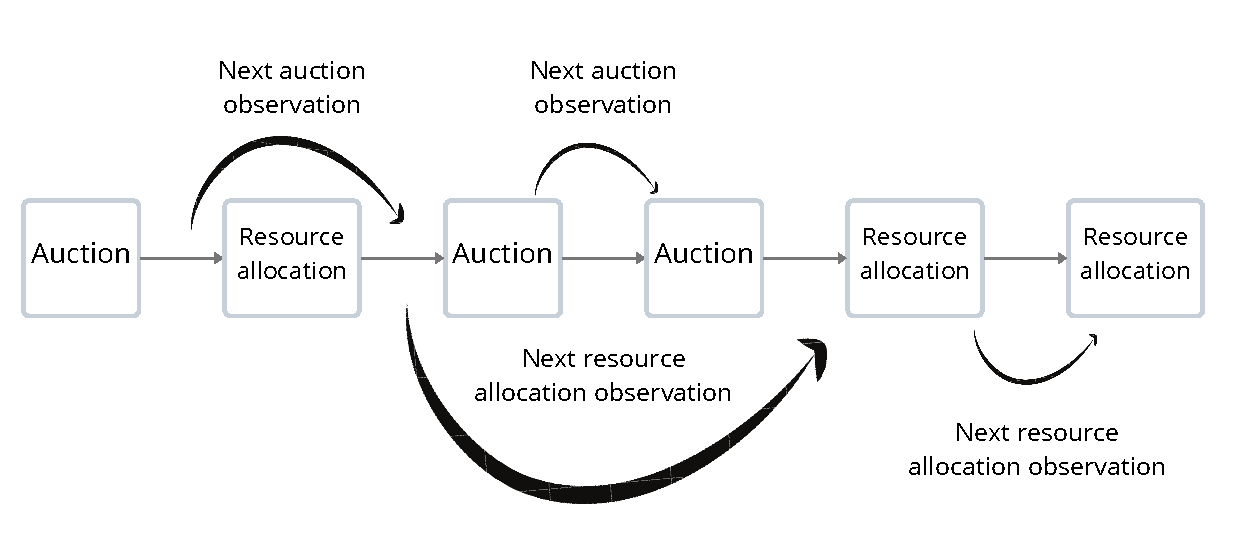
\includegraphics[width=14cm]{figures/4_implementation_figs/env_server_agents_observations.pdf}
    \caption{Environment server agents observations}
    \label{fig:environment-observations}
\end{figure}

For the resource allocation agent, a trick is implemented such that the next observation for the agent is not the
actual next resource allocation observation as shown in Figure~\ref{fig:environment-observations}. Instead a generated
observation from the resulting server state is used. This is identical to the last case in the figure
where no auction occurs between resource allocation steps. The resource allocation Q value is therefore able to
approximate the reward from its actions no matter the number of auctions that occur between
resource allocation steps.
% Todo add number of tasks observations problems

For the auction agent, the agent's observations require an auction task to select an action (the task bidding price).
Therefore a trick like the one implemented for the resource allocation agent can't be used in this case. Thus during
training, each server's last observation is recorded, to be used with the next auction observation. But this is a
suboptimal solution for the agent as the next observation has an unknown number of resource allocation steps between
them. A possible solution that has not been implement in this project is n step prediction~\citep{multi-step-dqn}.
This heuristic modifies the discounted reward to be n steps in the future. This approach could help
reduce the amount of randomness in the server's observations and improve bidding performance.

\section{Training Agents}
\label{sec:training-agents}
The first section of this chapter implementation simulations for MEC servers
(section~\ref{sec:simulating-mec-networks}) as a Reinforcement Learning environment. While the second
section implements auction and resource allocation agents that can interact with the proposed environment. This allows
for the training of agents using a range of algorithms outlined in Table~\ref{tab:reinforcement_learning_algorithms}.

Neural networks, the basis of the Reinforcement Learning agents implemented, often require huge amounts of data and
high powered Graphical Processing Unit (GPU) to run efficiently. Because of this, Iridis 5, University of Southampton's
supercomputer was utilised with GTX1050 GPUs to train these agents for long periods of time and en mass. During training,
for each episode a random environment was generated from a list of possible environment settings.

After every 10 episodes, the agents would be evaluated using a set of environments that are pre-generated and
saved at the beginning of training. This allowed the same environments to be used between training agents in order to
have a consistent basis to compare the agents over time.

To ensure that agents explored the state space as much as possible, during training actions are taken randomly to allow
the agents to "explore". This is a key problem within Reinforcement learning, the exploration vs exploitation
dilemma~\citep{Sutton1998}. For the Dqn agents, including the Double Dqn, Dueling Dqn and Categorical Dqn, epsilon
greedy actions were taken such that a percentage of the actions are taken random. The exploration factor (epsilon) is
initially set at 1 and ending at 0.1 with it linearly decreasing over 100,000 actions. For the Ddpg and Td3 agents,
initially Gaussian distribution was used to add randomness to actions~\citep{ddpg}. However this was found to be
ineffective, due to half of the actions added a negative value to the action which is unhelpful as actions must be
positive. As a result, agents were found to only bid zero in all auctions. Therefore Gamma
distribution~\citep{gamma-distribution} was used with a constant shape parameter of 1 and the scale parameter linearly
decreasing from 4.5 to 0.5 over 100,000 actions. However further research is required as agents are found to instead
bid on every task.

A table of agent hyperparameters used in training can be found in \hyperref[app:agent-hyperparameter]{Appendix C}.

